\documentclass{if-beamer}
\begin{document}
	
	\title[Campus Formoso do Araguaia]{Curso FIC -- Mulheres Mil}
	\subtitle{Planilha eletrônica}
	\author{Gilmar Gomes do Nascimento}
	\institute[IFTO]{
		Instituto Federal do Tocantins\\
		Campus Formoso do Araguaia
	}
	\date{\today}
	\logo{
		
\includegraphics[scale=0.0085]{logo.jpg}
	}
	\subject{Servers} % metadata
	
	\graphicspath{{figuras/}}
	%---------------------------------------------------------------------------------
	\begin{frame}
		\titlepage
	\end{frame}
	
	\begin{frame}{Anúncio}
		\begin{figure}
			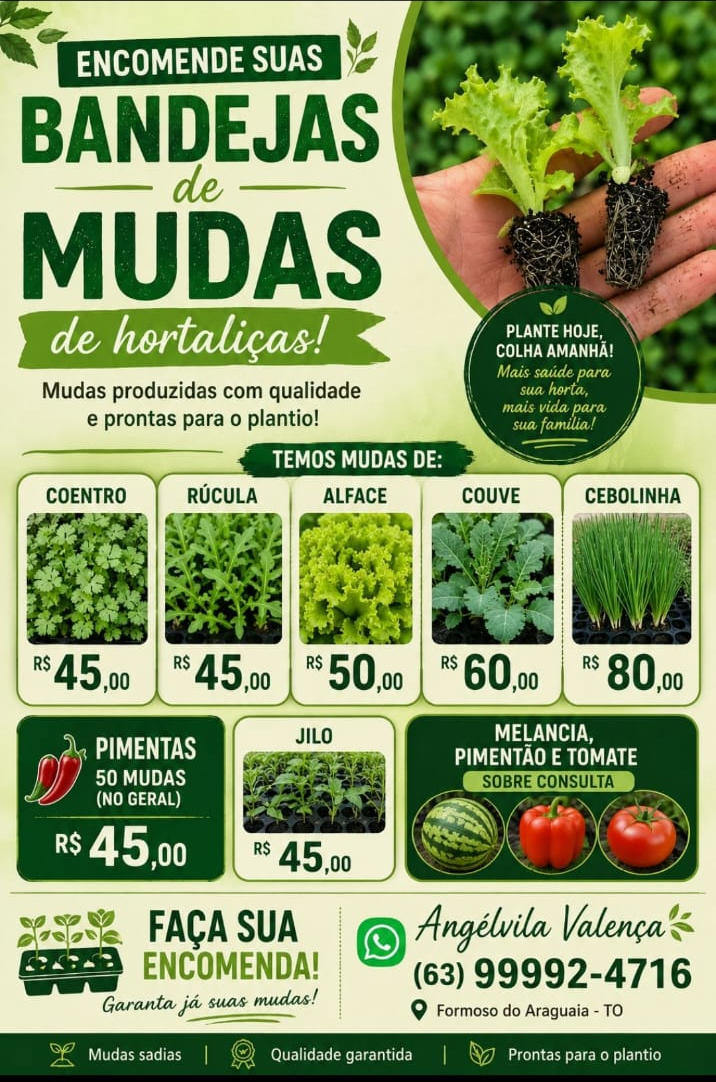
\includegraphics[scale=0.8]{bandeja}
		\end{figure}
	\end{frame}
	
	\begin{frame}{Planilha eletrônica}
	\begin{itemize}
		\item Abrir o LibreOffice Calc
		\item Digitar na Coluna A os hortaliças
		\item Digitar na Coluna B os preços
		\item Ordenar as hortaliças em ordem alfabética
		\item Inserir o cabeçalho com o título: Hortaliça da ``seu nome"~ e células mescladas
		\item Inserir uma linha com nome, preço, quantidade
		\item Inserir uma coluna com o identificador da hortaliça
		\item Salve a planilha com o nome Hortaliça
	\end{itemize}
	\end{frame}
	
	\begin{frame}{Vendas} 
	\begin{itemize}
		\item Crie as colunas Data, código produto, valor total, forma de pagamento
		\item Insira as vendas da hortaliça conforme orientação acima
		\item Na coluna forma de pagamento use a opção ``Validação de dados" e insira as opções: PIX, crédito, débito, Fiado
		\item Faça a soma total da coluna valor total
		\item Simule que 2\% das vendas precisam ser poupados
	\end{itemize}
	
	\end{frame}
\end{document}
